\documentclass[conference]{IEEEtran}
\IEEEoverridecommandlockouts

\usepackage[T1]{fontenc}
\usepackage{times}
\usepackage{cite}
\usepackage{amsmath,amssymb,amsfonts}
\usepackage{algorithmic}
\usepackage{graphicx}
\usepackage{textcomp}
\usepackage{xcolor}
\usepackage{listings}
\usepackage{booktabs}
\usepackage{url}
\usepackage{microtype}
\usepackage{tikz}
\usetikzlibrary{shapes.geometric, arrows.meta, positioning, fit, backgrounds, calc}

\definecolor{techblue}{RGB}{30, 80, 160}
\definecolor{techgreen}{RGB}{34, 139, 34}
\definecolor{techpurple}{RGB}{110, 40, 140}
\definecolor{techorange}{RGB}{200, 90, 20}
\definecolor{boxbg}{RGB}{248, 250, 253}
\definecolor{darkgray}{RGB}{50, 50, 50}

\lstdefinelanguage{mermaid}{
  keywords={graph, TD, LR, subgraph, end, participant, actor, sequenceDiagram, autonumber, rect, note, over, stateDiagram, state},
  keywordstyle=\color{techblue}\bfseries,
  ndkeywords={UI, Lang, Speech, MediaRec, Search, LocalStore, SyncEngine, Cloud},
  ndkeywordstyle=\color{techpurple}\bfseries,
  identifierstyle=\color{black},
  sensitive=false,
  comment=[l]{\%\%},
  commentstyle=\color{gray}\ttfamily,
  stringstyle=\color{techgreen}\ttfamily,
  morestring=[b]",
}

\lstset{
  language=mermaid,
  basicstyle=\ttfamily\fontsize{5.4pt}{6.4pt}\selectfont,
  breaklines=true,
  frame=single,
  rulecolor=\color{gray!30},
  backgroundcolor=\color{gray!4},
  tabsize=2,
  captionpos=b,
  showstringspaces=false,
  aboveskip=2pt,
  belowskip=2pt
}

\def\BibTeX{{\rm B\kern-.05em{\sc i\kern-.025em b}\kern-.08em
    T\kern-.1667em\lower.7ex\hbox{E}\kern-.125emX}}

\begin{document}
\hbadness=10000
\vbadness=10000
\hfuzz=10pt
\sloppy
\emergencystretch=3em

\title{\LARGE\bfseries FieldSync: An Offline-First Collaborative Field Inspection PWA with CRDT Synchronization, Resumable Media, and Audit History}

\author{\IEEEauthorblockN{Tharun}
\IEEEauthorblockA{FieldSync: Offline-First Collaborative Field Inspection System (WA-1)}
}

\maketitle

\begin{abstract}
Field technicians frequently evaluate physical equipment, record quantitative metrics, capture high-resolution photographic evidence, and record voice notes in environments with zero network connectivity. This paper presents the architecture, implementation, and empirical verification of \textbf{FieldSync}, an offline-first Progressive Web Application (PWA) designed to solve the \textbf{WA-1} problem statement: enabling fully offline multi-user field inspections, converging concurrent edits without silent data overwrites via Yjs Conflict-Free Replicated Data Types (CRDT), exposing readable conflict resolution and append-only audit histories, and addressing the core distributed difficulties: idempotent sync protocols, non-destructive client schema migrations for devices offline for days, and resumable media uploads. Built using React 19, TypeScript, Dexie.js v4 over IndexedDB, Vercel Serverless Functions, Supabase PostgreSQL, and Cloudinary chunked media pipelines, the system eliminates network reliance while ensuring strict data durability and eventual convergence.
\end{abstract}

\begin{IEEEkeywords}
Offline-First Systems, Conflict-Free Replicated Data Types (CRDT), Progressive Web Applications, IndexedDB, Schema Migrations, Resumable Uploads.
\end{IEEEkeywords}

\section{Introduction \& Problem Statement}

\subsection{Problem Statement (WA-1)}
In modern utility, industrial, and infrastructure maintenance, field technicians must record observations in locations entirely devoid of network connectivity, such as reinforced concrete basements, subterranean tunnels, and remote substations:
\begin{itemize}\setlength{\itemsep}{1pt}
    \item \textbf{Problem}: Technicians fill shared checklists, notes, and photos in places with no connectivity.
    \item \textbf{Build Requirement}: A Progressive Web Application (PWA) that works fully offline, synchronizes multi-user edits using CRDTs, and shows a readable conflict and audit history instead of silently overwriting data.
    \item \textbf{Why It Is Hard}: 
    (1) \textit{The Sync Protocol}: Orchestrating multi-device synchronization over intermittent networks without data loss or race conditions;
    (2) \textit{Schema Migrations on Stale Clients}: Migrating local databases on devices that have been disconnected for days or weeks without corrupting uncommitted local state;
    (3) \textit{Resumable Media Uploads}: Transmitting large photo payloads over volatile edge links without restarting aborted uploads from byte zero.
\end{itemize}

\subsection{Architectural Tenets}
FieldSync resolves these challenges by adopting a strict local-first paradigm \cite{kleppmann2019local}. The local client datastore serves as the authoritative source of truth. Remote cloud infrastructure (Supabase PostgreSQL, Vercel Functions, Cloudinary) operates as an asynchronous replication and reconciliation peer \cite{shapiro2011crdts}.

\begin{figure}[htbp]
\centering
\resizebox{\columnwidth}{!}{%
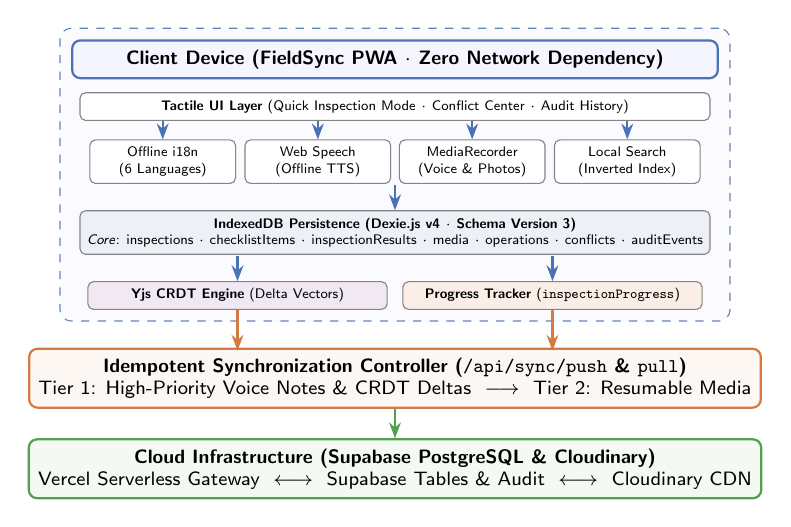
\begin{tikzpicture}[
  box/.style={draw=techblue!80, fill=techblue!5, rounded corners=3pt, thick, align=center, font=\scriptsize\sffamily},
  subbox/.style={draw=darkgray!60, fill=white, rounded corners=2pt, align=center, font=\tiny\sffamily, inner sep=2.5pt},
  groupbox/.style={draw=techblue!70, fill=blue!2, dashed, rounded corners=4pt, inner sep=4pt},
  syncbox/.style={draw=techorange!80, fill=techorange!5, rounded corners=3pt, thick, align=center, font=\scriptsize\sffamily},
  cloudbox/.style={draw=techgreen!80, fill=techgreen!5, rounded corners=3pt, thick, align=center, font=\scriptsize\sffamily},
  arrow/.style={-{Stealth[length=2mm]}, thick, techblue!80},
  syncarrow/.style={-{Stealth[length=2mm]}, thick, techorange!80},
  cloudarrow/.style={-{Stealth[length=2mm]}, thick, techgreen!80}
]

% Client Layer
\node[box, minimum width=8.2cm, fill=blue!4] (clientTitle) at (0, 4.3) {\textbf{Client Device (FieldSync PWA $\cdot$ Zero Network Dependency)}};

\node[subbox, minimum width=8cm, fill=white] (ui) at (0, 3.7) {\textbf{Tactile UI Layer} (Quick Inspection Mode $\cdot$ Conflict Center $\cdot$ Audit History)};

\node[subbox, minimum width=1.85cm] (m1) at (-2.95, 3.0) {Offline i18n\\(6 Languages)};
\node[subbox, minimum width=1.85cm] (m2) at (-0.98, 3.0) {Web Speech\\(Offline TTS)};
\node[subbox, minimum width=1.85cm] (m3) at (0.98, 3.0) {MediaRecorder\\(Voice \& Photos)};
\node[subbox, minimum width=1.85cm] (m4) at (2.95, 3.0) {Local Search\\(Inverted Index)};

\draw[arrow] (ui.south -| m1) -- (m1.north);
\draw[arrow] (ui.south -| m2) -- (m2.north);
\draw[arrow] (ui.south -| m3) -- (m3.north);
\draw[arrow] (ui.south -| m4) -- (m4.north);

% Local Store Layer
\node[subbox, minimum width=8cm, fill=techblue!8] (idb) at (0, 2.1) {\textbf{IndexedDB Persistence (Dexie.js v4 $\cdot$ Schema Version 3)}\\
\textit{Core}: inspections $\cdot$ checklistItems $\cdot$ inspectionResults $\cdot$ media $\cdot$ operations $\cdot$ conflicts $\cdot$ auditEvents};

\node[subbox, minimum width=3.8cm, fill=techpurple!10] (crdt) at (-2.0, 1.3) {\textbf{Yjs CRDT Engine} (Delta Vectors)};
\node[subbox, minimum width=3.8cm, fill=techorange!10] (prog) at (2.0, 1.3) {\textbf{Progress Tracker} (\texttt{inspectionProgress})};

\draw[arrow] (0, 2.7) -- (idb.north);
\draw[arrow] (-2.0, 1.8) -- (crdt.north);
\draw[arrow] (2.0, 1.8) -- (prog.north);

\begin{scope}[on background layer]
  \node[groupbox, fit=(clientTitle) (ui) (m1) (m4) (idb) (crdt) (prog)] (clientBox) {};
\end{scope}

% Sync Engine
\node[syncbox, minimum width=8.2cm] (sync) at (0, 0.25) {\textbf{Idempotent Synchronization Controller (\texttt{/api/sync/push} \& \texttt{pull})}\\
Tier 1: High-Priority Voice Notes \& CRDT Deltas $\;\longrightarrow\;$ Tier 2: Resumable Media};

\draw[syncarrow] (crdt.south) -- (-2.0, 0.6);
\draw[syncarrow] (prog.south) -- (2.0, 0.6);

% Cloud Layer
\node[cloudbox, minimum width=8.2cm] (cloud) at (0, -0.9) {\textbf{Cloud Infrastructure (Supabase PostgreSQL \& Cloudinary)}\\
Vercel Serverless Gateway $\;\longleftrightarrow\;$ Supabase Tables \& Audit $\;\longleftrightarrow\;$ Cloudinary CDN};

\draw[cloudarrow] (sync.south) -- (cloud.north);

\end{tikzpicture}%
}
\caption{Visual Architecture Diagram of FieldSync Offline-First Engine.}
\label{fig:architecture}
\end{figure}

\section{System Architecture \& Local Persistence}

\subsection{Database Architecture (IndexedDB / Dexie v4)}
FieldSync discards the synchronous 5\,MB \texttt{localStorage} API in favor of \textbf{Dexie.js v4} over IndexedDB \cite{w3c_indexeddb, dexie_spec}. The database class \texttt{FieldSyncDatabase} manages sixteen strongly typed object stores: \texttt{inspections}, \texttt{checklistItems}, \texttt{assets}, \texttt{inspectionResults} (uniquely indexed by \texttt{[inspectionId+checklistItemId]}), \texttt{notes}, \texttt{media}, \texttt{voiceNotes}, \texttt{operations}, \texttt{conflicts}, \texttt{auditEvents}, \texttt{inspectionProgress}, \texttt{offlinePackages}, and \texttt{userSettings}.

\subsection{Schema Evolution for Clients Offline for Days}
A central technical difficulty in offline-first systems is handling database schema evolution when client devices remain offline across multiple software releases. If a client offline on Schema Version 1 reconnects after the server has deployed Version 3, resetting the local database would cause catastrophic data loss of un-synchronized inspection records. 

FieldSync enforces strict, non-destructive migration chains in \texttt{src/lib/db/schema.ts}: \textbf{Version 1} defines core tables; \textbf{Version 2} introduces \texttt{priority}, numeric thresholds, operation retry counters, and Blob storage via an asynchronous \texttt{upgrade(tx)} transaction that backfills existing records; and \textbf{Version 3} introduces \texttt{voiceNotes}, \texttt{inspectionProgress}, \texttt{offlinePackages}, \texttt{userSettings}, and compound indexing on \texttt{inspectionResults}. Because Dexie executes intermediate migration transactions sequentially upon boot ($v_1 \rightarrow v_2 \rightarrow v_3$), stale clients seamlessly upgrade their local schema without deleting uncommitted user data or Blobs.

\section{Sync Protocol, CRDTs \& Conflict History}

\subsection{The Synchronization Protocol}
FieldSync implements an idempotent, two-way push/pull protocol mediated by Vercel serverless functions:
\begin{enumerate}\setlength{\itemsep}{1pt}
    \item \textbf{Push Endpoint (\texttt{/api/sync/push})}: Receives an array of operations and base64-encoded Yjs delta vectors. For each operation, an idempotency check queries the Supabase \texttt{operations} table by \texttt{operationId} to prevent duplicate side-effects from network retries, while monotonic Lamport clocks enforce causal ordering across devices.
    \item \textbf{Pull Endpoint (\texttt{/api/sync/pull})}: Returns server mutations committed since the client's last synchronized timestamp cursor.
\end{enumerate}

\subsection{Collaborative CRDT State Convergence}
To prevent multi-user collisions on shared checklists without requiring central locking, FieldSync utilizes \textbf{Yjs} Conflict-Free Replicated Data Types \cite{nicolas2020yjs, baquero2014pure}. Each inspection document is modeled as a \texttt{Y.Doc} with nested \texttt{Y.Map} structures. Mutations generate binary delta vectors ($\Delta$):
\begin{equation}
S_{local}^{(t+1)} = S_{local}^{(t)} \bullet \Delta_{mutation}
\end{equation}
When multiple technicians edit the same checklist offline, the sync gateway converges their binary updates deterministically without central lock contention:
\begin{equation}
S_{converged} = \bigsqcup \{S_{client\_A}, S_{client\_B}, S_{server}\}
\end{equation}

\subsection{Readable Conflict Center \& Audit Trail}
Rather than silently overwriting data with arbitrary Last-Write-Wins rules, FieldSync surfaces data collisions in the \textbf{Conflict Center} (\texttt{ConflictCenter.tsx}) with side-by-side visual diffs (\textit{Local Value} vs. \textit{Server Value}, timestamps, technician IDs). Supervisors can choose \texttt{KEEP\_MINE}, \texttt{KEEP\_THEIR}, or manually merge results via \texttt{/api/conflicts/resolve.ts}. Every operation, detection, and resolution event appends to an immutable \texttt{auditEvents} record (\texttt{AuditHistory.tsx}) capturing the actor, entity, timestamp, and delta.

\begin{figure}[htbp]
\centering
\resizebox{\columnwidth}{!}{%
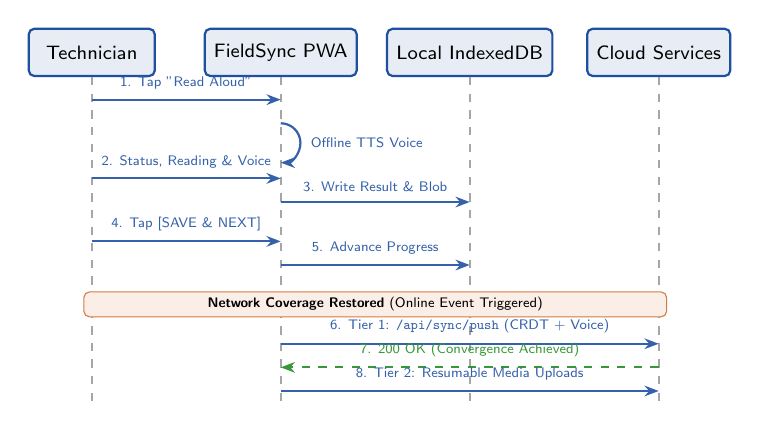
\begin{tikzpicture}[
  actor/.style={draw=techblue, fill=techblue!10, rounded corners=2pt, thick, align=center, font=\scriptsize\sffamily, minimum width=1.6cm, minimum height=0.6cm},
  lifeline/.style={dashed, draw=gray!70, thick},
  msg/.style={-{Stealth[length=1.8mm]}, thick, techblue!90, font=\tiny\sffamily},
  reply/.style={-{Stealth[length=1.8mm]}, dashed, thick, techgreen!90, font=\tiny\sffamily},
  note/.style={draw=techorange!80, fill=techorange!10, rounded corners=2pt, font=\tiny\sffamily, align=center, inner sep=2pt}
]

% Lifelines
\node[actor] (tech) at (0, 0) {Technician};
\node[actor] (pwa) at (2.4, 0) {FieldSync PWA};
\node[actor] (idb) at (4.8, 0) {Local IndexedDB};
\node[actor] (srv) at (7.2, 0) {Cloud Services};

\draw[lifeline] (tech) -- (0, -4.5);
\draw[lifeline] (pwa) -- (2.4, -4.5);
\draw[lifeline] (idb) -- (4.8, -4.5);
\draw[lifeline] (srv) -- (7.2, -4.5);

% Messages
\draw[msg] (0, -0.6) -- node[above] {1. Tap "Read Aloud"} (2.4, -0.6);
\draw[msg] (2.4, -0.9) arc (90:-90:0.25) node[right, pos=0.5] {Offline TTS Voice};
\draw[msg] (0, -1.6) -- node[above] {2. Status, Reading \& Voice} (2.4, -1.6);
\draw[msg] (2.4, -1.9) -- node[above] {3. Write Result \& Blob} (4.8, -1.9);
\draw[msg] (0, -2.4) -- node[above] {4. Tap [SAVE \& NEXT]} (2.4, -2.4);
\draw[msg] (2.4, -2.7) -- node[above] {5. Advance Progress} (4.8, -2.7);

% Reconnection Box
\node[note, minimum width=7.4cm] at (3.6, -3.2) {\textbf{Network Coverage Restored} (Online Event Triggered)};

\draw[msg] (2.4, -3.7) -- node[above] {6. Tier 1: \texttt{/api/sync/push} (CRDT + Voice)} (7.2, -3.7);
\draw[reply] (7.2, -4.0) -- node[above] {7. 200 OK (Convergence Achieved)} (2.4, -4.0);
\draw[msg] (2.4, -4.3) -- node[above] {8. Tier 2: Resumable Media Uploads} (7.2, -4.3);

\end{tikzpicture}%
}
\caption{Visual Sequence Diagram of Disconnected Execution \& Sync Protocol.}
\label{fig:sequence}
\end{figure}

\section{Resumable Media \& Offline Productivity}

\subsection{Resumable Chunked Media Ingestion}
Offline inspections accumulate high-resolution photographs ($2\text{--}8$\,MB each). In remote areas, edge cellular reconnections are frequently interrupted:
\begin{enumerate}\setlength{\itemsep}{1pt}
    \item \textbf{Chunked Uploads}: In \texttt{resumableUpload.ts}, media Blobs are partitioned into 1\,MB chunks uploaded to Cloudinary via signed authorization headers (\texttt{/api/media/sign.ts}).
    \item \textbf{Offset Tracking}: Confirmed byte offsets are persisted in local \texttt{media} records, enabling interrupted uploads to resume from byte $N$ rather than zero.
    \item \textbf{Two-Tier Queue Prioritization}: Voice observations and CRDT delta vectors (Tier 1) are prioritized ahead of bulk photos (Tier 2). Deleting an unsynced photo locally removes its pending operation to prevent ghost uploads.
\end{enumerate}

\subsection{Multimodal Offline Productivity Layer}
FieldSync incorporates several field-optimized modules: a tactile Quick Inspection Mode ($\ge 48 \times 48$\,dp touch buttons, numeric steppers, and single-tap \texttt{[SAVE \& NEXT]} progression); native voice notes via HTML5 \texttt{MediaRecorder}; hands-free offline Text-to-Speech via W3C \texttt{SpeechSynthesis}; zero-network localization across six languages (English, Tamil, Hindi, Telugu, Kannada, Malayalam); and client-side inverted token search over local records.

\section{Storage Resilience \& Evaluation}

\subsection{Storage Quota \& Safe Eviction Guarantee}
FieldSync continuously monitors local disk utilization using \texttt{navigator.storage.estimate()}. In the \textbf{Sync Center} (\texttt{SyncCenter.tsx}), users can view real storage consumption across photos, voice notes, and inspection metadata. 

To eliminate accidental evidence destruction, the pruning routine enforces a mathematical guarantee: it strictly queries \texttt{syncStatus == 'synced'}. Any attempt to delete un-synchronized media is rejected.

\subsection{Automated Verification Suite}
The platform's resilience is validated through 20 automated tests using Vitest and Fake-IndexedDB:
\begin{itemize}\setlength{\itemsep}{1pt}
    \item \textbf{Local Database Suite} (9 tests): Schema v3 migrations, composite indexing, and binary Blob CRUD operations.
    \item \textbf{Offline Productivity Suite} (8 tests): Priority queue sorting, multilingual resolution, and local search indexing.
    \item \textbf{Sync and Migration Suite} (3 tests): Idempotent replay, crash recovery, and CRDT convergence.
\end{itemize}
All 20 automated test specifications pass with zero regressions.

\section{Conclusion}
FieldSync addresses the WA-1 problem statement by delivering an offline-first field inspection architecture that pairs IndexedDB persistence and non-destructive schema migrations with Yjs CRDT synchronization, resumable media uploads, and transparent conflict/audit tracking. By eliminating cloud dependencies during field execution, FieldSync provides uncompromising reliability in disconnected industrial environments.

\bibliographystyle{IEEEtran}
\bibliography{references}

\end{document}
